\section{Risultati}\label{risultati}
Il framework~\cite{benchmark}, oltre a contenere l'implementazione di alcuni algoritmi di inversione polinomiale
(tra cui la versione di partenza dell'algoritmo di Bernstein-Yang), fornisce dei tool per testare la performance dei
vari algoritmi per poi compararli; sono stati effettuati diversi test durante lo sviluppo, ma per brevità riportiamo solo
i risultati dell'implementazione originale e quella finale.
Ogni test prevede l'esecuzione di 1000 round per ogni $p$ di interesse; in ogni round viene misurato il tempo di esecuzione
dell'algoritmo, prima con un input casuale, poi con un trinomio ($x^2+x+1$):\footnote{In ogni caso, l'inversione
viene calcolata prendendo come modulo $x^{p}-1$} questo viene fatto per calcolare la t
di Student per le due popolazioni e verificare
che il tempo di esecuzione degli algoritmi sia costante in funzione dell'input (non della sua dimensione), garantendo che
il crittosistema che lo usa sia immune (in questo punto) ad attacchi \textit{side channel} che puntano a risalire all'input
analizzando i tempi di esecuzione.

I test sono stati effettuati su una macchina AMD64, con processore AMD Ryzen 5 2500U (disabilitando il TurboBoost e
bloccando la frequenza a 1.9GHz per ottenere risultati consistenti); l'implementazione è stata compilata con GCC 10.2.0, 
abilitando la generazione di codice specifico per l'architettura utilizzata (\texttt{-march=native}) e abilitando il livello
massimo di ottimizzazione (\texttt{-O3}).

\begin{figure}
    \centering
    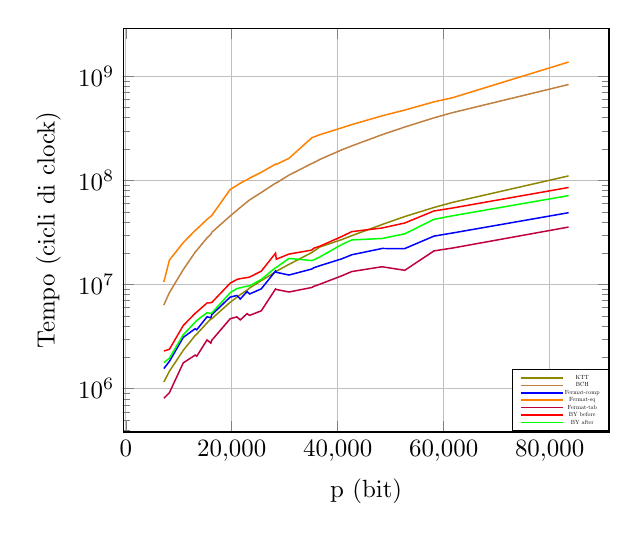
\begin{tikzpicture}[scale=0.9]
        \pgfplotsset{every axis/.append style={semithick}, legend style={nodes={scale=0.7, transform shape}, at={(1,0)},anchor=south east}}

	\begin{semilogyaxis}[
		xlabel=p (bit),ylabel=Tempo (cicli di clock), grid=major, xticklabel style={
            /pgf/number format/fixed,
            /pgf/number format/precision=5
            }, scaled x ticks=false ]

    \addplot[no marks, color=olive] coordinates{
        (7187, 1159197.4)
        (8237, 1469920.2)
        (10853, 2336473.4)
        (13109, 3246316.8)
        (13397, 3347390.0)
        (15331, 4277250.6)
        (16067, 4695806.2)
        (16229, 4694091.6)
        (19709, 6764716.4)
        (20981, 7556269.0)
        (21611, 8000344.2)
        (22901, 8858165.2)
        (23371, 9267820.8)
        (25579, 10906522.6)
        (28277, 13221080.6)
        (28411, 13423327.6)
        (30803, 15622464.4)
        (35117, 20323059.0)
        (35507, 20936273.0)
        (36629, 22957209.2)
        (40787, 27063629.4)
        (42677, 29510000.0)
        (48371, 37725077.4)
        (52667, 45033239.4)
        (58171, 54986958.0)
        (61717, 61625946.6)
        (83579, 110553683.6)
    };
    \addlegendentry{KTT}

    \addplot[no marks, color=brown] coordinates{
        (7187, 6368874.4)
        (8237, 8364095.6)
        (10853, 13922595.2)
        (13109, 20491931.0)
        (13397, 21293264.8)
        (15331, 28056795.4)
        (16067, 30382587.2)
        (16229, 31722889.2)
        (19709, 45575386.6)
        (20981, 51657051.6)
        (21611, 54956980.4)
        (22901, 62186967.6)
        (23371, 64996685.6)
        (25579, 76589311.4)
        (28277, 94263290.2)
        (28411, 94610992.2)
        (30803, 112420385.4)
        (35117, 145454923.6)
        (35507, 148202625.6)
        (36629, 158941209.0)
        (40787, 196929065.2)
        (42677, 214790361.0)
        (48371, 274893671.4)
        (52667, 325854983.0)
        (58171, 399131155.0)
        (61717, 448249901.0)
        (83579, 834007747.8)
    };
    \addlegendentry{BCH}

    \addplot[no marks, color=blue] coordinates {
        (7187, 1561699.8)
        (8237, 1827586.0)
        (10853, 3110983.6)
        (13109, 3770875.2)
        (13397, 3678711.8)
        (15331, 4900348.2)
        (16067, 4806660.2)
        (16229, 5133151.8)
        (19709, 7576635.0)
        (20981, 7857809.2)
        (21611, 7268007.2)
        (22901, 8562007.6)
        (23371, 8120296.6)
        (25579, 9097204.4)
        (28277, 13504138.2)
        (28411, 13120726.4)
        (30803, 12347247.6)
        (35117, 14105630.4)
        (35507, 14518979.4)
        (36629, 15177688.2)
        (40787, 17682828.6)
        (42677, 19342802.0)
        (48371, 22206770.4)
        (52667, 22177420.0)
        (58171, 29189824.2)
        (61717, 31306422.6)
        (83579, 48987526.4)
    };
    \addlegendentry{Fermat-comp}

    \addplot[no marks, color=orange] coordinates{
        (7187, 10597590.4)
        (8237, 17184007.0)
        (10853, 25297424.2)
        (13109, 33119433.8)
        (13397, 34034539.2)
        (15331, 42226171.0)
        (16067, 45221734.2)
        (16229, 46011999.6)
        (19709, 81895383.8)
        (20981, 89587471.2)
        (21611, 94080496.0)
        (22901, 101717262.2)
        (23371, 105224090.2)
        (25579, 119787535.4)
        (28277, 143408586.6)
        (28411, 142583988.2)
        (30803, 163023836.2)
        (35117, 256737134.2)
        (35507, 261421235.4)
        (36629, 274770918.6)
        (40787, 320387425.4)
        (42677, 343968765.2)
        (48371, 417034409.0)
        (52667, 474298878.0)
        (58171, 568372615.0)
        (61717, 623609013.0)
        (83579, 1370972271.0)        
    };
    \addlegendentry{Fermat-sq}
    
    \addplot[no marks, color=purple] coordinates {
        (7187, 809715.8)
        (8237, 915526.2)
        (10853, 1771415.4)
        (13109, 2103486.2)
        (13397, 2047749.8)
        (15331, 2939877.8)
        (16067, 2740291.6)
        (16229, 2917695.0)
        (19709, 4695404.2)
        (20981, 4895648.2)
        (21611, 4576126.0)
        (22901, 5257624.8)
        (23371, 5057833.2)
        (25579, 5597524.4)
        (28277, 9083607.2)
        (28411, 8978193.0)
        (30803, 8485064.2)
        (35117, 9378049.2)
        (35507, 9621184.2)
        (36629, 10076641.2)
        (40787, 12150942.0)
        (42677, 13344390.2)
        (48371, 14827613.0)
        (52667, 13711557.0)
        (58171, 21056187.8)
        (61717, 22448997.0)
        (83579, 35664757.6)        
    };
    \addlegendentry{Fermat-tab}

    \addplot[no marks, color=red] coordinates {
		(7187, 2301133.4)
        (8237, 2390625.0)
        (10853, 4044599.2)
        (13109, 5300937.4)
        (13397, 5446870.6)
        (15331, 6648405.6)
        (16067, 6702943.8)
        (16229, 6724461.8)
        (19709, 10310837.6)
        (20981, 11196952.2)
        (21611, 11407319.0)
        (22901, 11667615.0)
        (23371, 11805428.0)
        (25579, 13449986.4)
        (28277, 20024899.6)
        (28411, 17511886.6)
        (30803, 19631753.0)
        (35117, 21432919.4)
        (35507, 22369455.6)
        (36629, 23348801.4)
        (40787, 28987888.4)
        (42677, 32262773.2)
        (48371, 34922057.2)
        (52667, 39038512.2)
        (58171, 50907356.2)
        (61717, 54401236.2)
        (83579, 85570203.0)
    };
    \addlegendentry{BY before}

    \addplot[no marks, color=green] coordinates {
        (7187, 1782584.6)
        (8237, 1962955.5)
        (10853, 3299358.6)
        (13109, 4362019.9)
        (13397, 4522305.42)
        (15331, 5368479.5)
        (16067, 5286806.16)
        (16229, 5325745.7)
        (19709, 8352941.2)
        (20981, 9162305.2)
        (21611, 9307480.6)
        (22901, 9655103.68)
        (23371, 9723034.62)
        (25579, 11202767.42)
        (28277, 14555232.2)
        (28411, 14622453.44)
        (30803, 17820851.56)
        (35117, 17008580.68)
        (35507, 17287261.4)
        (36629, 18419434.4)
        (40787, 24264261.8)
        (42677, 26849432.52)
        (48371, 27695913.8)
        (52667, 30734590.3)
        (58171, 42328589.2)
        (61717, 45814829.52)
        (83579, 71488995.4)        
    };
    \addlegendentry{BY after}

    \end{semilogyaxis}%
\end{tikzpicture}%
\caption{Tempi di esecuzione}
\end{figure}
\begin{figure}
        \centering
\pgfplotsset{every axis/.append style={semithick}, legend style={nodes={scale=0.7, transform shape}, at={(1,0)},anchor=south east}}
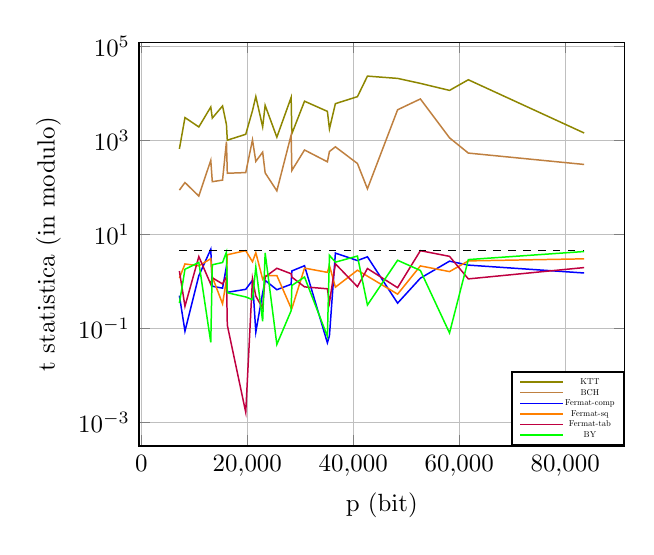
\begin{tikzpicture}[scale=0.9]
	\begin{semilogyaxis}[
        xlabel=p (bit),ylabel=t statistica (in modulo), grid=major, xticklabel style={
            /pgf/number format/fixed,
            /pgf/number format/precision=5
            }, scaled x ticks=false ]

        \addplot[no marks, color=olive] coordinates {
            (7187, 652.005696)
            (8237, 3019.920377)
            (10853, 1910.771944)
            (13109, 5071.778073)
            (13397, 2946.893161)
            (15331, 5332.226134)
            (16067, 2139.75731)
            (16229, 998.246284)
            (19709, 1332.526004)
            (20981, 4239.90178)
            (21611, 8454.250835)
            (22901, 1920.498214)
            (23371, 5492.804618)
            (25579, 1155.64429)
            (28277, 8096.484658)
            (28411, 1371.076919)
            (30803, 6732.774469)
            (35117, 4094.864009)
            (35507, 1734.952881)
            (36629, 5973.390682)
            (40787, 8408.629239)
            (42677, 23009.76453)
            (48371, 20572.562632)
            (52667, 16117.718704)
            (58171, 11429.139155)
            (61717, 19250.383818)
            (83579, 1419.418492)
    };
    \addlegendentry{KTT}
    
    \addplot[no marks, color=brown] coordinates {
            (7187, 86.646338)
            (8237, 125.408114)
            (10853, 64.681601)
            (13109, 372.819976)
            (13397, 130.796415)
            (15331, 141.441714)
            (16067, 928.621171)
            (16229, 197.779837)
            (19709, 204.312264)
            (20981, 1011.501825)
            (21611, 353.268775)
            (22901, 554.996088)
            (23371, 201.444914)
            (25579, 83.641382)
            (28277, 1285.511342)
            (28411, 226.541613)
            (30803, 617.673131)
            (35117, 346.507444)
            (35507, 573.58292)
            (36629, 720.523447)
            (40787, 318.858938)
            (42677, 92.41314)
            (48371, 4425.944718)
            (52667, 7515.104843)
            (58171, 1120.57332)
            (61717, 531.092093)
            (83579, 304.239061)
    };
    \addlegendentry{BCH}
    
    \addplot[no marks, color=blue] coordinates {
            (7187, 0.493086)
            (8237, 0.08653)
            (10853, 1.309049)
            (13109, 4.778504)
            (13397, 0.782128)
            (15331, 0.71157)
            (16067, 2.079124)
            (16229, 0.580534)
            (19709, 0.672241)
            (20981, 1.0493)
            (21611, 0.083094)
            (22901, 0.567385)
            (23371, 1.04121)
            (25579, 0.660099)
            (28277, 0.861794)
            (28411, 1.653982)
            (30803, 2.134661)
            (35117, 0.048959)
            (35507, 0.06948)
            (36629, 3.96631)
            (40787, 2.752093)
            (42677, 3.304725)
            (48371, 0.341822)
            (52667, 1.160096)
            (58171, 2.671217)
            (61717, 2.201135)
            (83579, 1.496464)
    };
    \addlegendentry{Fermat-comp}
    
    \addplot[no marks, color=orange] coordinates {
            (7187, 1.162409)
            (8237, 2.330743)
            (10853, 2.12729)
            (13109, 3.016198)
            (13397, 1.238996)
            (15331, 0.330162)
            (16067, 1.078995)
            (16229, 3.658359)
            (19709, 4.467738)
            (20981, 2.591605)
            (21611, 4.04695)
            (22901, 1.106657)
            (23371, 1.312441)
            (25579, 1.322171)
            (28277, 0.266311)
            (28411, 0.262227)
            (30803, 1.901191)
            (35117, 1.544098)
            (35507, 2.154404)
            (36629, 0.747209)
            (40787, 1.713264)
            (42677, 1.281831)
            (48371, 0.530638)
            (52667, 2.117118)
            (58171, 1.600775)
            (61717, 2.704511)
            (83579, 2.992715)
    };
    \addlegendentry{Fermat-sq}
    
    \addplot[no marks, color=purple] coordinates {
            (7187, 1.646462)
            (8237, 0.293479)
            (10853, 3.342243)
            (13109, 0.860273)
            (13397, 1.182994)
            (15331, 0.875522)
            (16067, 1.25272)
            (16229, 0.116413)
            (19709, 0.001627)
            (20981, 1.131281)
            (21611, 0.481985)
            (22901, 0.268159)
            (23371, 1.231348)
            (25579, 1.886799)
            (28277, 1.441204)
            (28411, 1.222019)
            (30803, 0.758732)
            (35117, 0.690352)
            (35507, 0.351563)
            (36629, 2.346714)
            (40787, 0.764265)
            (42677, 1.863431)
            (48371, 0.727855)
            (52667, 4.463352)
            (58171, 3.378872)
            (61717, 1.119912)
            (83579, 1.95091)
    };
    \addlegendentry{Fermat-tab}
    
    \addplot[no marks, color=green] coordinates {
            (7187, 0.342964)
            (8237, 1.79303)
            (10853, 2.511967)
            (13109, 0.05001)
            (13397, 2.238948)
            (15331, 2.499593)
            (16067, 4.175354)
            (16229, 0.568396)
            (19709, 0.462919)
            (20981, 0.405652)
            (21611, 2.010867)
            (22901, 0.140311)
            (23371, 4.014809)
            (25579, 0.045285)
            (28277, 0.236084)
            (28411, 0.81202)
            (30803, 1.22736)
            (35117, 0.06737)
            (35507, 3.550464)
            (36629, 2.543941)
            (40787, 3.429449)
            (42677, 0.312068)
            (48371, 2.789529)
            (52667, 1.693412)
            (58171, 0.0794)
            (61717, 2.885019)
            (83579, 4.281391)
    };
    \addlegendentry{BY}

    \addplot[no marks, color=black, style=dashed] coordinates {
        (7187, 4.5)
        (83579, 4.5)
    };
    

    \end{semilogyaxis}%
\end{tikzpicture}%
\caption{Valori della t di Student}
\end{figure}
\begin{figure}
    \centering
\pgfplotsset{every axis/.append style={semithick}, legend style={nodes={scale=0.7, transform shape}, at={(1,0)},anchor=south east}}
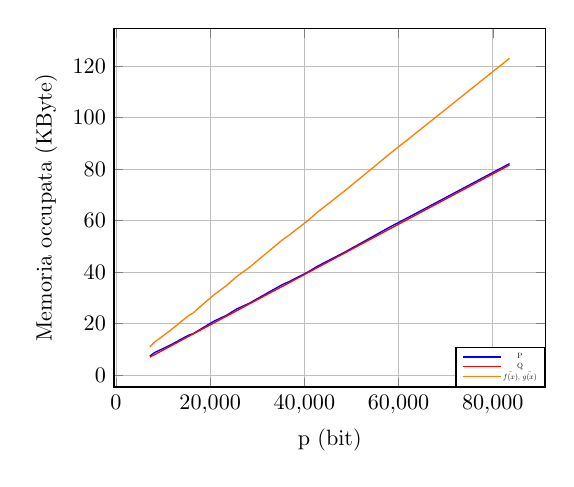
\begin{tikzpicture}[scale=0.8]
\begin{axis}[
    xlabel=p (bit),ylabel=Memoria occupata (KByte), grid=major, ticklabel style={
        /pgf/number format/fixed,
        /pgf/number format/precision=5
        }, scaled ticks=false ]

    \addplot[no marks, color=blue] coordinates {
        (7187, 7.375)
        (8237, 8.75)
        (10853, 11.0)
        (13109, 13.125)
        (13397, 13.5)
        (15331, 15.375)
        (16067, 15.875)
        (16229, 15.875)
        (19709, 19.71875)
        (20981, 21.09375)
        (21611, 21.59375)
        (22901, 22.71875)
        (23371, 23.09375)
        (25579, 25.59375)
        (28277, 27.84375)
        (28411, 27.96875)
        (30803, 30.46875)
        (35117, 34.90625)
        (35507, 35.28125)
        (36629, 36.15625)
        (40787, 40.03125)
        (42677, 42.15625)
        (48371, 47.53125)
        (52667, 51.875)
        (58171, 57.5)
        (61717, 60.875)
        (83579, 82.125)               
    };
    \addlegendentry{P}

    \addplot[no marks, color=red] coordinates {
        (7187, 6.9375)
        (8237, 7.9375)
        (10853, 10.5)
        (13109, 12.71875)
        (13397, 13.0)
        (15331, 14.90625)
        (16067, 15.625)
        (16229, 15.78125)
        (19709, 19.1875)
        (20981, 20.40625)
        (21611, 21.03125)
        (22901, 22.3125)
        (23371, 22.75)
        (25579, 24.90625)
        (28277, 27.5625)
        (28411, 27.6875)
        (30803, 30.03125)
        (35117, 34.21875)
        (35507, 34.59375)
        (36629, 35.6875)
        (40787, 39.78125)
        (42677, 41.625)
        (48371, 47.1875)
        (52667, 51.40625)
        (58171, 56.78125)
        (61717, 60.25)
        (83579, 81.5625)        
    };
    \addlegendentry{Q}

    \addplot[no marks, color=orange] coordinates {
        (7187, 10.9375)
        (8237, 12.84375)
        (10853, 16.375)
        (13109, 19.59375)
        (13397, 20.109375)
        (15331, 22.9375)
        (16067, 23.796875)
        (16229, 23.875)
        (19709, 29.421875)
        (20981, 31.421875)
        (21611, 32.234375)
        (22901, 33.984375)
        (23371, 34.59375)
        (25579, 38.171875)
        (28277, 41.734375)
        (28411, 41.921875)
        (30803, 45.59375)
        (35117, 52.15625)
        (35507, 52.71875)
        (36629, 54.140625)
        (40787, 60.046875)
        (42677, 63.09375)
        (48371, 71.25)
        (52667, 77.6875)
        (58171, 86.0)
        (61717, 91.109375)
        (83579, 123.046875)           
    };
    \addlegendentry{$\bar{f(x)}$, $\bar{g(x)}$}
\end{axis}%
\end{tikzpicture}%
\caption{Memoria occupata}
\end{figure}



Analizzando i risultati, notiamo che la \textit{nuova} versione dell'algoritmo di Bernstein-Yang ha un miglioramento
dal punto di vista temporale quasi costante per tutti i valori di $p$ (+18.56\%), rimanendo più lento dell'algoritmo
KTT~\cite{takagi2001fast} per $p < 35507$ (rispetto a $p < 48371$ della versione originale); d'altro canto, i valori della t di Student per BY sono inferiori in modulo a 4.5, la 
soglia sotto cui possiamo affermare che il tempo di esecuzione dell'algoritmo è indipendente dall'input con un
livello di confidenza del 99.999\%, a differenza di KTT. 


